\documentclass[11pt,a4paper]{article}

\usepackage[margin=2.4cm]{geometry}
\usepackage[T1]{fontenc}
\usepackage{lmodern}
\usepackage{amsmath,amssymb,amsfonts,bm,mathtools}
\usepackage{booktabs,array,tabularx}
\usepackage{enumitem}
\usepackage{xcolor}
\usepackage{tikz}
\usetikzlibrary{shapes.geometric,arrows.meta,positioning,calc}
\usepackage[colorlinks=true,linkcolor=blue!50!black,urlcolor=blue!50!black]{hyperref}
\usepackage{fancyhdr}
\usepackage{microtype}
\usepackage[strings]{underscore}

\setlist{itemsep=2pt,topsep=4pt}
\setlength{\parindent}{0pt}
\setlength{\parskip}{5pt}
\pagestyle{fancy}
\fancyhf{}
\fancyhead[L]{\small\itshape DroneSim: Technical Reconstruction}
\fancyhead[R]{\small\thepage}

% ---------- notation ----------
\newcommand{\R}{\mathbb{R}}
\newcommand{\vc}[1]{\bm{#1}}
\newcommand{\ez}{\vc{e}_z}
\newcommand{\norm}[1]{\left\lVert #1\right\rVert}
\newcommand{\abs}[1]{\left\lvert #1\right\rvert}
\newcommand{\dd}{\mathrm{d}}
\newcommand{\code}[1]{\texttt{\small #1}}
\newcommand{\hatv}[1]{\widehat{#1}}
\DeclareMathOperator{\clip}{clip}
\DeclareMathOperator{\sgn}{sgn}
\DeclareMathOperator{\tr}{tr}
\DeclareMathOperator{\diag}{diag}
\DeclareMathOperator{\sd}{sd}

\title{\vspace{-1.2cm}\textbf{Vision-Cued Minimum-Jerk Collision Avoidance for a\\
Wind-Perturbed Quadrotor:}\\[4pt]
\large A Mathematical and Algorithmic Reconstruction of the \textsc{DroneSim} Pipeline\\
--- Rigid-Body Dynamics, Geometric Cascaded Control, Disturbance Observation,\\
Ornstein--Uhlenbeck Gust Synthesis and Monocular Time-to-Contact Estimation}
\author{Technical report derived from source-code analysis of the\\
\emph{Drone Navigator Telemetry System} repository}
\date{\today}

\begin{document}
\maketitle
\thispagestyle{fancy}

\begin{abstract}
\noindent
This report documents, equation by equation, what the simulator in the repository \emph{actually} computes.
It is based on the source (\code{dronesim/}, \code{frontend/src}, \code{tests/}) and not on the README, which describes
only an early prototype (a YOLO heads-up display with a heuristic distance $d = 3000/(h_{\text{box}}+1)$).
The current system is a full pipeline: a monocular video is passed through a detector/tracker; the apparent growth of
the tracked bounding box gives a time-to-contact (TTC) and, with an assumed physical size and a pinhole camera model, a metric
range, closing speed and lateral offset; these define a static-obstacle scenario; a sampling-based planner chooses a
minimum-jerk detour (or a braking stop) subject to acceleration, thrust and tilt limits that include aerodynamic
drag in a steady 3-D wind; and a cascaded geometric flight controller with a Luenberger disturbance observer tracks the
plan through a 17-state, RK4-integrated quadrotor model with four first-order rotors, in a world that may contain
seeded Ornstein--Uhlenbeck turbulence. The result is recorded in a deterministic JSON schema and replayed in a
web front end. All parameters are \emph{assumed}, not measured; the report flags these assumptions and lists
observed limitations in the final section.
\end{abstract}

\tableofcontents
\newpage

%=====================================================================
\section{Scope, Provenance and the State of the README}
%=====================================================================
The repository contains two generations of code.

\begin{description}[leftmargin=0.5cm,style=nextline]
\item[Generation 1 (legacy; what the README describes).] \code{object\_detection\_for\_rescue\_operations.py}
runs YOLOv8 on each frame, draws boxes, declares a target ``\textsc{locked}'' when the box centre lies in the middle 20\,\% of the
image ($0.4W<c_x<0.6W$), and displays a \emph{heuristic} distance
\begin{equation}
\hatv{d}\;=\;\operatorname{round}\!\Bigl(\frac{3000}{(y_2-y_1)+1},\,1\Bigr)\ \text{``m''},
\label{eq:legacy-dist}
\end{equation}
which is an uncalibrated inverse-proportional mapping (the constant $3000$ has units px$\cdot$m and is not derived from any
camera model). There is no dynamics, planning or control.
\item[Generation 2 (current; \code{dronesim/}).] A physically-based pipeline with no scripted motion: the only way
the virtual drone moves is by applying four motor commands to the rigid-body model (\code{Quadrotor.step}).
\end{description}

This report concerns Generation 2. Section~\ref{sec:limits} lists the points where the code departs from what a casual reading of
the README (or of some docstrings) would suggest.

%=====================================================================
\section{System Architecture}
%=====================================================================
\subsection{End-to-end data flow}

\begin{figure}[h]
\centering
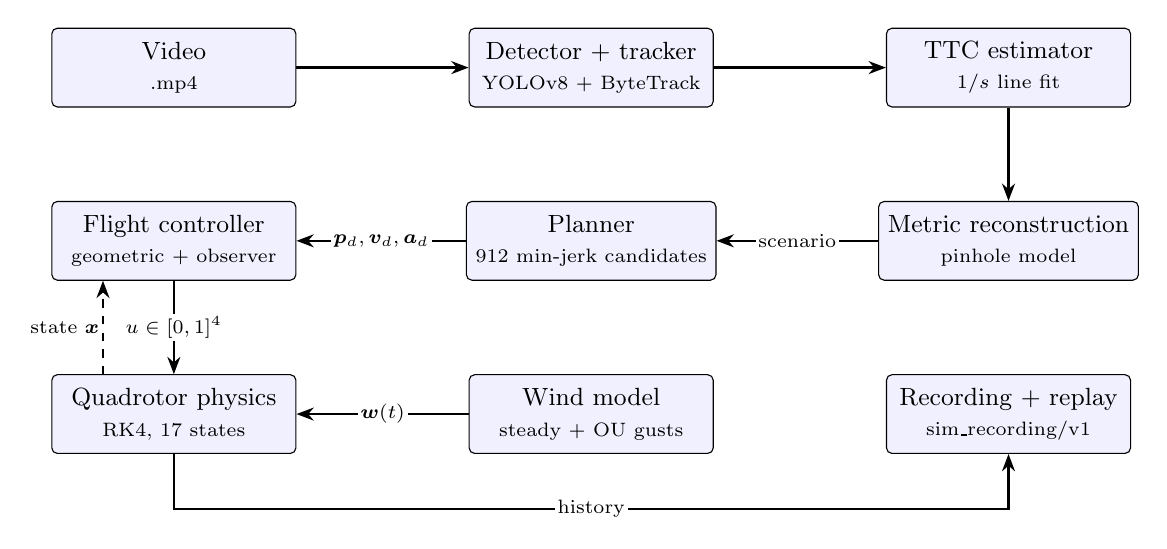
\begin{tikzpicture}[
  blk/.style={draw,rounded corners=2pt,align=center,minimum width=3.1cm,minimum height=1.0cm,font=\small,fill=blue!6},
  arr/.style={-{Stealth[length=2.2mm]},thick},
  lab/.style={font=\scriptsize,fill=white,inner sep=1pt}]
\node[blk] (vid) at (0,0) {Video\\{\scriptsize .mp4}};
\node[blk] (det) at (5.3,0) {Detector + tracker\\{\scriptsize YOLOv8 + ByteTrack}};
\node[blk] (est) at (10.6,0) {TTC estimator\\{\scriptsize $1/s$ line fit}};
\node[blk] (rec) at (10.6,-2.2) {Metric reconstruction\\{\scriptsize pinhole model}};
\node[blk] (plan) at (5.3,-2.2) {Planner\\{\scriptsize 912 min-jerk candidates}};
\node[blk] (ctrl) at (0,-2.2) {Flight controller\\{\scriptsize geometric + observer}};
\node[blk] (phys) at (0,-4.4) {Quadrotor physics\\{\scriptsize RK4, 17 states}};
\node[blk] (wind) at (5.3,-4.4) {Wind model\\{\scriptsize steady + OU gusts}};
\node[blk] (recd) at (10.6,-4.4) {Recording + replay\\{\scriptsize sim\_recording/v1}};
\draw[arr] (vid)--(det);
\draw[arr] (det)--(est);
\draw[arr] (est)--(rec);
\draw[arr] (rec)--(plan) node[lab,pos=0.5]{scenario};
\draw[arr] (plan)--(ctrl) node[lab,pos=0.5]{$\vc p_d,\vc v_d,\vc a_d$};
\draw[arr] (ctrl.south)--(phys.north) node[lab,pos=0.5]{$u\in[0,1]^4$};
\draw[arr] (wind)--(phys) node[lab,pos=0.5]{$\vc w(t)$};
\draw[arr] (phys.south) -- ++(0,-0.7) -| (recd.south) node[lab,pos=0.25]{history};
\draw[arr,dashed] ([xshift=-0.9cm]phys.north) -- ([xshift=-0.9cm]ctrl.south) node[lab,pos=0.5,left]{state $\vc x$};
\end{tikzpicture}
\caption{Pipeline. Solid arrows: data flow. Dashed: the controller reads the true simulated state (no sensor noise).}
\end{figure}

\subsection{Module map}
\begin{center}
\small
\begin{tabularx}{\textwidth}{@{}l>{\raggedright\arraybackslash}X@{}}
\toprule
Module & Role \\ \midrule
\code{config.py} & Dataclasses for vision, obstacle size and camera FOV (all flagged \emph{assumed}). \\
\code{vision/detector.py} & YOLO + tracker wrapper; yields detections with $t=\text{frame}/\text{fps}$. \\
\code{vision/obstacle\_estimator.py} & Bounding box $\to$ size signal $s=\sqrt{wh}$, TTC and growth by least squares. \\
\code{vision/reconstruction.py} & Pixels $\to$ metres (range, lateral, vertical, closing speed); builds the scenario. \\
\code{vision/export.py} & Target-track selection, writes \code{obstacle\_track.json}. \\
\code{sim/params.py} & Drone parameters and derived constants ($k_T,k_M$, hover command, motor layout). \\
\code{sim/quaternion.py} & $[w,x,y,z]$ quaternion algebra, Euler conversions. \\
\code{sim/motors.py} & Command$\to\omega\to$ thrust/torque/power maps; mixer matrix. \\
\code{sim/quadrotor.py} & 17-state dynamics, RK4, zero-order-hold command. \\
\code{sim/wind.py} & Steady wind vector + seeded Ornstein--Uhlenbeck gusts. \\
\code{sim/collision.py} & Box signed distance, clearance, collision prediction. \\
\code{sim/planner.py} & Min-jerk detour/brake candidate generation, wind-aware feasibility, cost. \\
\code{sim/controller.py} & Cascaded controller, disturbance observer, desaturating mixer. \\
\code{sim/loop.py} & Multi-rate closed-loop driver (physics $500$\,Hz, control $250$\,Hz). \\
\code{sim/runner.py} & Plan $\to$ fly $\to$ verify $\to$ re-plan; summaries. \\
\code{sim/recording.py} & JSON schema, random-access \code{Replay}. \\
\code{api/app.py} & FastAPI service: runs, video, re-simulation without re-running YOLO, async processing jobs. \\
\code{frontend/src/*} & React/Three.js replay (HUD, motor graphs, wind widgets); TypeScript port of \code{Replay}. \\
\bottomrule
\end{tabularx}
\end{center}

\subsection{Execution sequence}
The CLI chain (also invoked by the API as three subprocesses) is
\begin{enumerate}[label=(\roman*)]
\item \code{python -m dronesim.vision.export VIDEO} $\to$ \code{obstacle\_track.json} (schema \code{obstacle\_track/v1});
\item \code{python -m dronesim.vision.reconstruction obstacle\_track.json} $\to$ \code{obstacle\_metric.json} (\code{obstacle\_metric/v1});
\item \code{python -m dronesim.run\_scenario obstacle\_metric.json [wind, dodge, \dots]} $\to$ \code{sim\_recording.json} (\code{sim\_recording/v1}).
\end{enumerate}
The API endpoint \code{POST /api/runs/\{run\}/simulate} redoes only step (iii) with new settings, so YOLO is never re-run.

%=====================================================================
\section{Conventions and Notation}
%=====================================================================
\begin{itemize}
\item \textbf{World frame} $\mathcal W$ (ENU-like): $+x$ is the drone's initial forward / approach axis, $+y$ is left, $+z$ is up.
\item \textbf{Body frame} $\mathcal B$ (FLU): $+x$ forward, $+y$ left, $+z$ up.
\item \textbf{Camera frame}: $+Z$ forward (range), $+X$ right, $+Y$ up. The conversion to the world frame is
$(Z,X,Y)\mapsto(x,-y,z)$, i.e.\ camera-right becomes world $-y$.
\item \textbf{Quaternion} $\vc q=[q_w,q_x,q_y,q_z]^\top$, unit, rotating body vectors to world vectors: $\vc v_{\mathcal W}=\vc R(\vc q)\vc v_{\mathcal B}$.
\item \textbf{Euler angles}: ZYX (yaw--pitch--roll) in radians.
\end{itemize}

\begin{table}[h]
\centering\small
\begin{tabular}{@{}ll@{\qquad}ll@{}}
\toprule
Symbol & Meaning & Symbol & Meaning \\ \midrule
$\vc p,\vc v$ & position, velocity in $\mathcal W$ & $\vc\omega$ & body angular velocity \\
$\vc R,\vc q$ & body$\to$world rotation / quaternion & $\Omega_i$ & rotor $i$ speed (rad/s) \\
$m$ & mass & $\vc J$ & inertia matrix \\
$T_i$ & thrust of motor $i$ & $\vc w(t)$ & wind velocity in $\mathcal W$ \\
$c_d$ & quadratic drag coefficient (kg/m) & $\vc d$ & disturbance (drag) acceleration \\
$k_T,k_M$ & thrust / torque coefficients & $u_i\in[0,1]$ & normalised motor command \\
$\vc F$ & desired force vector & $g$ & $9.80665$\,m/s$^2$ \\
\bottomrule
\end{tabular}
\caption{Principal symbols.}
\end{table}

\subsection{Quaternion algebra (\code{quaternion.py})}
Hamilton product for $\vc a=[a_w,\vc a_v]$, $\vc b=[b_w,\vc b_v]$:
\[
\vc a\otimes\vc b=\bigl[a_wb_w-\vc a_v\!\cdot\!\vc b_v,\; a_w\vc b_v+b_w\vc a_v+\vc a_v\times\vc b_v\bigr].
\]
Rotation matrix:
\begin{equation}
\vc R(\vc q)=\begin{bmatrix}
1-2(q_y^2+q_z^2) & 2(q_xq_y-q_zq_w) & 2(q_xq_z+q_yq_w)\\
2(q_xq_y+q_zq_w) & 1-2(q_x^2+q_z^2) & 2(q_yq_z-q_xq_w)\\
2(q_xq_z-q_yq_w) & 2(q_yq_z+q_xq_w) & 1-2(q_x^2+q_y^2)
\end{bmatrix}.
\end{equation}
Euler $\to$ quaternion (half-angles $c_\bullet=\cos(\bullet/2)$, $s_\bullet=\sin(\bullet/2)$):
\begin{align*}
q_w&=c_rc_pc_y+s_rs_ps_y, & q_x&=s_rc_pc_y-c_rs_ps_y,\\
q_y&=c_rs_pc_y+s_rc_ps_y, & q_z&=c_rc_ps_y-s_rs_pc_y.
\end{align*}
Quaternion $\to$ Euler:
\begin{align}
\phi&=\operatorname{atan2}\bigl(2(q_wq_x+q_yq_z),\,1-2(q_x^2+q_y^2)\bigr),\\
\theta&=\arcsin\!\bigl(\clip(2(q_wq_y-q_zq_x),-1,1)\bigr),\\
\psi&=\operatorname{atan2}\bigl(2(q_wq_z+q_xq_y),\,1-2(q_y^2+q_z^2)\bigr).
\end{align}
Rotation matrix $\to$ quaternion uses Shepperd's method: if $\tr\vc R>0$, $s=2\sqrt{\tr\vc R+1}$ and
$\vc q=\bigl[\tfrac s4,\tfrac{R_{32}-R_{23}}{s},\tfrac{R_{13}-R_{31}}{s},\tfrac{R_{21}-R_{12}}{s}\bigr]$; otherwise the largest diagonal element
$i$ is used (indices $j,k$ cyclic), $s=2\sqrt{R_{ii}-R_{jj}-R_{kk}+1}$, which keeps the divisor away from zero.

%=====================================================================
\section{Vision Front End: From Pixels to a Time-to-Contact}
%=====================================================================
\subsection{Detection and tracking}
\code{track\_video} runs \code{ultralytics.YOLO(yolov8s.pt).track(\dots, conf=0.3, tracker=bytetrack.yaml, persist=True)}.
The detection confidence threshold is $0.3$ (the legacy HUD used $0.6$) because a looming obstacle has low confidence at long range.
The class filter is empty by default, since the COCO label assigned to a plain box is arbitrary. Frame time is $t=i/\text{fps}$.

\subsection{Target-track selection}
The obstacle is taken to be the track with the largest accumulated bounding-box area,
\begin{equation}
\tau^\star=\arg\max_{\tau}\;\sum_{k}A_{\tau,k},\qquad A=(x_2-x_1)(y_2-y_1),
\end{equation}
on the grounds that a looming object dominates the view. All other tracks with $\ge10$ frames are reported (\code{other\_tracks}) but not used.

\subsection{Size signal}
For each frame in which track $\tau^\star$ is seen, the box width and height $w,h$ (pixels) give the scalar size
\begin{equation}
s=\sqrt{wh}\qquad(\text{with }wh\ge10^{-9}).
\end{equation}

\subsection{Time-to-contact from monocular expansion}
For a pinhole camera of focal length $f$ viewing a fronto-parallel object of true linear size $S$ at range $Z$,
the apparent size is $s=fS/Z$, i.e.\ $1/s=Z/(fS)$. If the closing speed $v_c=-\dot Z$ is approximately constant,
\begin{equation}
\frac1{s(t)}=\frac{Z_0-v_ct}{fS}\ \Longrightarrow\ \frac{\dd}{\dd t}\!\Bigl(\frac1s\Bigr)=-\frac{v_c}{fS},
\qquad
\boxed{\ \text{TTC}=\frac{Z}{v_c}=-\frac{1/s}{\dd(1/s)/\dd t}\ }
\label{eq:ttc}
\end{equation}
which is independent of $f$ and $S$ (pixels suffice). Differencing two box heights is noisy, so the code fits a straight line by
ordinary least squares (\code{np.polyfit}, degree 1) to $\{(t_k,1/s_k)\}$ over a sliding window of the last $T_w=0.75$\,s
(requiring $\ge5$ samples):
\[
\frac1{s}\approx\beta\,t+\alpha,\qquad \hatv{\beta}=\frac{\sum(t_k-\bar t)(\sigma_k-\bar\sigma)}{\sum(t_k-\bar t)^2},\ \ \sigma_k=1/s_k.
\]
Evaluating the fit at the latest time $t_n$, $\sigma_n=\hatv\beta t_n+\hatv\alpha$, gives
\begin{equation}
\text{TTC}=-\frac{\sigma_n}{\hatv\beta},\qquad
\dot s=-\frac{\hatv\beta}{\sigma_n^{2}}\quad(\text{since }\dot s=\tfrac{\dd}{\dd t}\sigma^{-1}=-\dot\sigma/\sigma^{2}).
\end{equation}
TTC is reported only if $\hatv\beta<0$ (approaching), $\sigma_n>0$ and $\text{TTC}\le30$\,s; otherwise it is ``not approaching'' (a near-zero slope is noise).
When the detector loses the object, the last fitted TTC is propagated for at most $T_{\text{gap}}=2$\,s:
\begin{equation}
\text{TTC}(t)=\max\bigl(0,\ \text{TTC}_{\text{last}}-(t-t_{\text{last}})\bigr),\qquad \text{source}=\text{``extrapolated''}.
\end{equation}

%=====================================================================
\section{Metric Reconstruction (Pinhole Model)}
%=====================================================================
\textbf{Assumptions (all configurable, none measured):} the real obstacle size $W\times H$ (default $0.5\times0.5$\,m, thickness $0.05$\,m) is supplied;
the camera looks level along the forward axis with no distortion; the horizontal FOV is nominal ($82.6^\circ$); the obstacle is fronto-parallel and static.

\subsection{Focal length in pixels}
For image width $W_{\text{img}}$ and horizontal FOV $\alpha$,
\begin{equation}
f=\frac{W_{\text{img}}/2}{\tan(\alpha/2)}.
\end{equation}

\subsection{Range, lateral and vertical offsets}
Width and height each give an independent range estimate, combined by their geometric mean:
\begin{equation}
Z_w=\frac{fW}{w},\quad Z_h=\frac{fH}{h},\quad Z=\sqrt{Z_wZ_h}=f\sqrt{\frac{WH}{wh}}=\frac{f\sqrt{WH}}{s}.
\end{equation}
With image centre $(c_{x0},c_{y0})=(W_{\text{img}}/2,H_{\text{img}}/2)$ and box centre $(\bar x,\bar y)$,
\begin{equation}
X=\frac{(\bar x-c_{x0})Z}{f}\ (\text{right}),\qquad Y=\frac{(c_{y0}-\bar y)Z}{f}\ (\text{up}),
\end{equation}
and the metric box size is $(wZ/f,\;hZ/f)$.

\subsection{Closing speed}
From $Z=k/s$ one gets $\dot Z=-Z\dot s/s$, hence the closing speed from the fitted growth rate $\dot s$ is
\begin{equation}
v_c=-\dot Z=\frac{Z\,\dot s}{s}.
\end{equation}
Consistency with \eqref{eq:ttc}: $Z/v_c=s/\dot s$, which equals $-\sigma_n/\hatv\beta$ since $\dot s=-\hatv\beta/\sigma_n^2$ and $s=1/\sigma_n$.
During detection gaps flagged ``extrapolated'', $Z(t)=\max(0,Z_0-v_0(t-t_0))$ with the last speed and lateral/vertical offsets held.

\subsection{Scenario construction}
The first $n_{\text{ref}}=12$ measured rows having a speed are taken and the \emph{median} (middle element of the sorted list) of range $Z_0$, closing speed $v_0$, lateral and vertical offsets is used:
\begin{align}
\text{drone}&:\ \vc p_0=(0,0,0),\ \vc v_0=(\max(v_0,0),0,0),\ \text{heading }+x,\\
\text{obstacle centre}&:\ (Z_0,\,-X_0,\,Y_0)\quad(\text{camera right}\to\text{world }-y),\\
\text{panel}&:\ \text{width }W,\ \text{height }H,\ \text{thickness }t_p\ \text{along }x,\ \text{normal }(-1,0,0),\\
\text{initial TTC}&:\ Z_0/v_0\ (\text{if }v_0>10^{-6}).
\end{align}
\textbf{Note.} The TTC of \S4.4 is carried through for display; the planner consumes $Z_0$ and $v_0$ (i.e.\ the same information) rather than TTC itself.

\subsection{Time scaling to the video}
If the user overrides the approach speed (e.g.\ for a faster demonstration), the recording stores a \code{time\_scale} $=v_{\text{video}}/v_{\text{sim}}$ so that video time is
$t_{\text{video}}=t_{\text{ref}}+\text{time\_scale}\cdot t_{\text{sim}}$ (\code{None} if not defined).

%=====================================================================
\section{Vehicle Model (\code{params.py}, \code{motors.py}, \code{quadrotor.py})}
%=====================================================================
\subsection{Parameters}
The values below are \emph{assumed, Tello-class orders of magnitude}, explicitly not a datasheet.

\begin{table}[h]
\centering\small
\begin{tabular}{@{}llr@{}}
\toprule
Quantity & Symbol & Value \\ \midrule
Mass & $m$ & $0.080$\,kg \\
Arm offset (X layout, along $x$ and $y$) & $d$ & $0.045$\,m \\
Inertia (diagonal) & $\diag(J_{xx},J_{yy},J_{zz})$ & $(1,1,2)\times10^{-4}$\,kg\,m$^2$ \\
Max rotor speed & $\Omega_{\max}$ & $1500$\,rad/s \\
Max thrust per motor & $T_{\max}$ & $0.40$\,N \\
Torque/thrust ratio & $\rho=k_M/k_T$ & $0.016$\,m \\
Rotor spin-axis inertia & $J_r$ & $2\times10^{-7}$\,kg\,m$^2$ \\
Motor time constant & $\tau_m$ & $0.03$\,s \\
Motor efficiency, idle power & $\eta,\;P_0$ & $0.7,\ 0.3$\,W \\
Quadratic drag coefficient & $c_d$ & $0.006$\,kg/m \\
Angular damping & $c_\omega$ & $2\times10^{-6}$\,N\,m\,s \\
Tilt / acceleration limits (controller and planner) & $\theta_{\max},a_{\max}$ & $35^\circ,\ 6$\,m/s$^2$ \\
\bottomrule
\end{tabular}
\caption{\code{DroneParams} defaults.}
\end{table}

Derived constants:
\begin{align}
k_T&=\frac{T_{\max}}{\Omega_{\max}^2}=1.778\times10^{-7}\ \text{N/(rad/s)}^2, & k_M&=\rho k_T=2.844\times10^{-9}\ \text{N\,m/(rad/s)}^2,\\
u_{\text{hover}}&=\sqrt{\frac{mg/4}{T_{\max}}}=0.700, & \Omega_{\text{hover}}&=u_{\text{hover}}\Omega_{\max}\approx1050\ \text{rad/s}.
\end{align}
The weight is $mg=0.7845$\,N, so the thrust-to-weight ratio is $4T_{\max}/(mg)\approx2.04$.

\subsection{Motor layout}
X configuration; positions $(x_i,y_i)$ and spin directions $s_i$ ($+1$ CCW seen from above, $-1$ CW):
\begin{center}\small
\begin{tabular}{@{}clccc@{}}
\toprule
$i$ & Position & $x_i$ & $y_i$ & $s_i$ \\ \midrule
1 & front--right & $+d$ & $-d$ & $+1$ \\
2 & rear--right & $-d$ & $-d$ & $-1$ \\
3 & rear--left & $-d$ & $+d$ & $+1$ \\
4 & front--left & $+d$ & $+d$ & $-1$ \\ \bottomrule
\end{tabular}
\end{center}

\subsection{Rotor and command model}
Four quantities are kept separate: command $u$, angular speed $\Omega$, thrust $T$ and electrical power $P$.
\begin{align}
u_i&\in[0,1]\ (\text{clipped}),\qquad \Omega_i^{\text{cmd}}=u_i\,\Omega_{\max}\quad(\text{linear map}),\label{eq:cmd}\\
\dot\Omega_i&=\frac{\Omega_i^{\text{cmd}}-\Omega_i}{\tau_m}\quad(\text{first-order lag}),\label{eq:lag}\\
T_i&=k_T\Omega_i^2,\qquad Q_i=k_M\Omega_i^2,\label{eq:TQ}\\
P_i&=\frac{Q_i\,\Omega_i}{\eta}+P_0.\label{eq:P}
\end{align}
Because \eqref{eq:cmd} is linear in $u$ and \eqref{eq:TQ} is quadratic in $\Omega$, steady-state thrust is $T_i=T_{\max}u_i^2$; the inverse used by the controller is
$u_i=\sqrt{\max(T_i,0)/T_{\max}}$ (clipped to $[0,1]$). At hover, $Q=3.14\times10^{-3}$\,N\,m and $P\approx5.0$\,W per motor ($\approx20$\,W total).
The rotor bandwidth is $1/\tau_m\approx33$\,rad/s.

\subsection{Rigid-body equations of motion}
The state is $\vc x=[\vc p,\vc v,\vc q,\vc\omega,\vc\Omega]\in\R^{17}$ ($3+3+4+3+4$).
Body torques from the rotors:
\begin{align}
\tau_x&=\sum_i y_iT_i,\qquad \tau_y=-\sum_i x_iT_i,\label{eq:tauxy}\\
\tau_z&=-\sum_i s_i\bigl(Q_i+J_r\dot\Omega_i\bigr).\label{eq:tauz}
\end{align}
The reaction torque on the body is opposite to the rotor spin; the $J_r\dot\Omega$ term is the reaction from accelerating the rotor.
Translational dynamics, with aerodynamic drag on the \emph{air-relative} velocity $\vc v_{\text{rel}}=\vc v-\vc w$:
\begin{equation}
m\dot{\vc v}=\vc R(\vc q)\begin{bmatrix}0\\0\\\sum_iT_i\end{bmatrix}-mg\,\ez-c_d\norm{\vc v_{\text{rel}}}\,\vc v_{\text{rel}},\qquad \dot{\vc p}=\vc v.
\label{eq:trans}
\end{equation}
Rotational dynamics (Euler's equation with linear damping) and kinematics:
\begin{equation}
\vc J\dot{\vc\omega}=\vc\tau-\vc\omega\times\vc J\vc\omega-c_\omega\vc\omega,\qquad
\dot{\vc q}=\tfrac12\,\vc q\otimes[0,\vc\omega].
\label{eq:rot}
\end{equation}
The drag law is quadratic; with $c_d=\tfrac12\rho_a C_dA$ the model corresponds to a lumped area--drag product. The drone's terminal free-fall speed is
$\sqrt{mg/c_d}\approx11.4$\,m/s.

\subsection{Numerical integration}
\code{Quadrotor.step(u)} performs one fixed step ($h=\Delta t=0.002$\,s) of classical fourth-order Runge--Kutta with the motor command held constant (zero-order hold):
\begin{align}
\vc k_1&=f(t,\vc x),& \vc k_2&=f(t+\tfrac h2,\vc x+\tfrac h2\vc k_1),\\
\vc k_3&=f(t+\tfrac h2,\vc x+\tfrac h2\vc k_2),& \vc k_4&=f(t+h,\vc x+h\vc k_3),\\
\vc x_{n+1}&=\vc x_n+\tfrac h6(\vc k_1+2\vc k_2+2\vc k_3+\vc k_4),
\end{align}
followed by renormalising $\vc q\leftarrow\vc q/\norm{\vc q}$. Time is $t=n\,\Delta t$ (an exact multiple of the step, independent of the wall clock). The wind function is evaluated at the stage times, so it must be a deterministic function of $t$. Logged outputs
(command, $\Omega$, $T$, $P$, body torque, acceleration, wind) are taken at the beginning of the step. The default initial rotor speeds are the hover speed (the drone starts airborne and in equilibrium).

\subsection{Mixer}
The steady-state map from per-motor thrusts to wrench $[F,\tau_x,\tau_y,\tau_z]^\top=\vc A[T_1,\dots,T_4]^\top$ is
\begin{equation}
\vc A=\begin{bmatrix}
1&1&1&1\\
y_1&y_2&y_3&y_4\\
-x_1&-x_2&-x_3&-x_4\\
-s_1\rho&-s_2\rho&-s_3\rho&-s_4\rho
\end{bmatrix}
=\begin{bmatrix}
1&1&1&1\\
-d&-d&d&d\\
-d&d&d&-d\\
-\rho&\rho&-\rho&\rho
\end{bmatrix}.
\end{equation}
(\code{thrusts\_from\_wrench} solves it numerically; it ignores the $J_r\dot\Omega$ term.) The rows are mutually orthogonal, with
$\vc A\vc A^\top=\diag(4,\,4d^2,\,4d^2,\,4\rho^2)$, so the inverse is analytic:
\begin{equation}
T_i=\frac F4+\frac{y_i\,\tau_x}{4d^2}-\frac{x_i\,\tau_y}{4d^2}-\frac{s_i\,\tau_z}{4\rho}
=\frac F4\pm\frac{\tau_x}{4d}\pm\frac{\tau_y}{4d}\mp\frac{\tau_z}{4\rho}.
\label{eq:mixinv}
\end{equation}

\subsection{Actuation authority (derived)}
Maximum roll/pitch torque (two motors at $T_{\max}$, two at 0) is $2dT_{\max}=0.036$\,N\,m, giving $\dot p_{\max}\approx360$\,rad/s$^2$;
maximum yaw torque is $2\rho T_{\max}=0.0128$\,N\,m, giving $\dot r_{\max}=64$\,rad/s$^2$. Yaw authority is therefore ${\sim}5.6\times$ weaker than roll/pitch,
which motivates the yaw-first sacrifice rule of \S\ref{sec:desat}.

%=====================================================================
\section{Wind Model (\code{wind.py})}
%=====================================================================
\subsection{Steady component}
With azimuth $\psi$ (from $+x$ toward $+y$) and elevation $\varepsilon$ (from the horizontal plane toward $+z$), and describing where the wind blows \emph{toward},
\begin{equation}
\vc w_0=V\begin{bmatrix}\cos\varepsilon\cos\psi\\\cos\varepsilon\sin\psi\\\sin\varepsilon\end{bmatrix}.
\end{equation}
Thus $\psi=0^\circ$ is a tailwind, $180^\circ$ a headwind, $+90^\circ$ blows toward the left, and $\varepsilon=90^\circ$ is a pure updraft. The inverse is
$V=\norm{\vc w}$, $\psi=\operatorname{atan2}(w_y,w_x)$, $\varepsilon=\arcsin(w_z/V)$. In the approach frame, headwind $=-w_x$, crosswind (left) $=w_y$, vertical $=w_z$.

\subsection{Turbulence: independent Ornstein--Uhlenbeck processes}
Each axis carries an OU (first-order Gauss--Markov) gust:
\begin{equation}
\dd X=-\frac{X}{\tau}\dd t+\sigma\sqrt{\frac2\tau}\,\dd W_t .
\end{equation}
Its exact discretisation over a step $\Delta$ is
\begin{equation}
X_{k+1}=a\,X_k+\sigma\sqrt{1-a^2}\,\xi_k,\qquad a=e^{-\Delta/\tau},\ \ \xi_k\sim\mathcal N(0,1),
\end{equation}
started from the stationary law $X_0\sim\mathcal N(0,\sigma^2)$. Therefore $\mathbb E[X]=0$, $\operatorname{Var}[X]=\sigma^2$ and the autocorrelation is
$R(\ell)=\sigma^2e^{-|\ell|/\tau}$ \emph{exactly}, independent of the sampling step $\Delta$ (here $\Delta=0.01$\,s). The corresponding one-sided power spectral density
is the Lorentzian $S(f)=\dfrac{4\sigma^2\tau}{1+(2\pi f\tau)^2}$; this is a simple Gauss--Markov gust model, \emph{not} the Dryden/von K\'arm\'an spectrum.
Defaults: $\tau=2$\,s, $\sigma=0$ (steady wind).

Implementation details that matter for reproducibility: the series is generated once on a fixed grid with a seeded \code{numpy.random.default_rng}
(draw order: stationary start, then the noise block), so a longer track extends a shorter one and the same seed gives the same gusts independent of the flight duration;
it is linearly interpolated, $X(t)=(1-\lambda)X_i+\lambda X_{i+1}$, and clamped outside $[0,t_{\max}]$.
The total wind is $\vc w(t)=\vc w_0+\vc X(t)$, which depends on time only (the argument \code{position} is ignored: there is no spatial shear).

%=====================================================================
\section{Collision Geometry (\code{collision.py})}
%=====================================================================
The obstacle is an axis-aligned box $\mathcal B$ with centre $\vc c$ and half extents $\vc h=\tfrac12[t_p,W,H]$ (thickness along $x$); the drone is a sphere of radius $r=0.10$\,m.
Signed distance to the box surface:
\begin{equation}
\vc q=\abs{\vc p-\vc c}-\vc h,\qquad
\operatorname{sd}(\vc p)=\norm{\max(\vc q,\vc 0)}+\min\bigl(\max_i q_i,0\bigr),
\end{equation}
positive outside, negative inside. Clearance is
\begin{equation}
\mathcal C(\vc p)=\min\Bigl(\operatorname{sd}(\vc p)-r,\ \ p_z-z_{\text{floor}}-r\Bigr).
\end{equation}
\code{predict\_collision} marks a \emph{collision} if $\mathcal C<0$ anywhere on the sampled path and a \emph{margin violation} if $\mathcal C<d_{\text{safe}}$ ($0.25$\,m), and reports first-event times and $\min\mathcal C$.
In the runner the obstacle's height $z$ is offset by the start altitude (default $1.5$\,m) so that it is level with the drone, and the floor is $z=0$.

%=====================================================================
\section{Avoidance Planner (\code{planner.py})}
%=====================================================================
The planner assumes the cruise heading is $+x$ at constant speed $v$. It works in the inertial frame, where the kinematics of the path are unaffected by wind;
wind only changes the force the rotors must supply.

\subsection{Minimum-jerk primitive}
The quintic with zero velocity and acceleration at both ends:
\begin{equation}
\sigma(\tau)=10\tau^3-15\tau^4+6\tau^5,\quad
\sigma'(\tau)=30\tau^2(1-\tau)^2,\quad
\sigma''(\tau)=60\tau-180\tau^2+120\tau^3,\qquad\tau\in[0,1].
\end{equation}
Peaks: $\max\sigma'=\sigma'(\tfrac12)=\tfrac{15}8$ and $\max\abs{\sigma''}=\tfrac{10}{\sqrt3}\approx5.77$.

\subsection{Nominal path and key times}
With start $\vc p_s$ and obstacle front/back planes $x_{\text{f}},x_{\text{b}}$ inflated by body radius and safety margin,
\begin{align}
x_{\text{f}}&=c_x-h_x-r-d_{\text{safe}}, & x_{\text{b}}&=c_x+h_x+r+d_{\text{safe}},\\
t_{\text{f}}&=\max\!\Bigl(\frac{x_{\text{f}}-p_{s,x}}{v},0\Bigr), & t_{\text{b}}&=\frac{x_{\text{b}}-p_{s,x}}{v}.
\end{align}
The straight path is $\vc p_{\text{nom}}(t)=\vc p_s+(vt,0,0)$, checked against the obstacle by \code{predict\_collision}. If it keeps the safety margin, no avoidance is needed.

\subsection{Detour family}
A detour offsets the nominal path by $D$ along a unit vector $\vc u(\phi)=(0,\cos\phi,\sin\phi)$ ($\phi=0$: $+y$ left, $90^\circ$: up), rises over $T_b$, holds, then returns:
\begin{align}
s(t)&=\sigma\!\Bigl(\frac{t-t_1}{T_b}\Bigr)-\sigma\!\Bigl(\frac{t-t_2}{T_b}\Bigr),\\
\vc p(t)&=\vc p_{\text{nom}}(t)+D\,s(t)\,\vc u,\quad
\vc v(t)=\vc v_{\text{nom}}+\frac{D}{T_b}\bigl[\sigma'_r-\sigma'_f\bigr]\vc u,\quad
\vc a(t)=\frac{D}{T_b^2}\bigl[\sigma''_r-\sigma''_f\bigr]\vc u,
\end{align}
with
\begin{equation}
t_1=\max(0,\;e\,t_{\text{f}}-T_b),\qquad t_2=t_{\text{b}}+0.3\ \text{s}.
\end{equation}
The peak lateral acceleration of a detour is $a_{\text{lat}}\approx D\cdot\tfrac{10}{\sqrt3}/T_b^2$ (e.g.\ $D=0.7$, $T_b=3$\,s: $0.45$\,m/s$^2$).

\textbf{Candidate grid.} $8$ directions $\phi\in\{0,45,\dots,315\}^\circ$ $\times$ $19$ offsets $D\in\{0.2,0.3,\dots,2.0\}$\,m $\times$ $3$ blend times $T_b\in\{1,2,3\}$\,s
$\times$ $2$ rise-end fractions $e\in\{0.6,0.9\}$ $=\mathbf{912}$ candidates, sampled every $\Delta t=0.02$\,s.

\subsection{Braking fallback}
If no detour is feasible, a minimum-jerk speed profile removes the full speed over $T$:
\begin{equation}
\dot x(t)=v\bigl(1-\sigma(t/T)\bigr),\quad
x(t)=v\Bigl[t-T\bigl(\tfrac52\tau^4-3\tau^5+\tau^6\bigr)\Bigr],\ \tau=\frac tT,\quad
a_x=-\frac{v}{T}\sigma'(\tau),
\end{equation}
using $\int_0^\tau\sigma=\tfrac52\tau^4-3\tau^5+\tau^6$. The stopping distance is $vT/2$ (since $\int_0^1\sigma=\tfrac12$), so $T=2\,d_{\text{avail}}\kappa/v$ with $\kappa\in\{1,0.9,0.8\}$ and $d_{\text{avail}}=x_{\text{f}}-p_{s,x}$.
Peak deceleration is $\tfrac{15}{8}v/T$. If this also fails, the result is ``unavoidable within limits'' and no avoidance flight is run.

\subsection{Wind-aware feasibility}
Air-relative drag acceleration is $\vc a_D=-(c_d/m)\norm{\vc v-\vc w}(\vc v-\vc w)$. To realise a planned inertial acceleration $\vc a_{\text{plan}}$, the rotors must supply
\begin{equation}
\vc a_{\text{req}}=\vc a_{\text{plan}}+\frac{c_d}{m}\norm{\vc v-\vc w}(\vc v-\vc w),\qquad
\vc f=\vc a_{\text{req}}+g\ez\ \ (\text{specific force}),
\end{equation}
and the limits are checked on this quantity (steady mean wind only):
\begin{align}
\text{accel: }&\max\norm{\vc a_{\text{req}}}\le\lambda a_{\max},\\
\text{thrust: }&m\max\norm{\vc f}\le\lambda\cdot4T_{\max},\\
\text{tilt: }&\max\arccos\bigl(f_z/\norm{\vc f}\bigr)\le\lambda\,\theta_{\max},
\end{align}
with $\lambda=0.8$ (\code{limit\_fraction}): effectively $4.8$\,m/s$^2$, $1.28$\,N and $28^\circ$. Clearance is checked on the plan with a required value
$d_{\text{safe}}+0.05\text{ m}+\delta_{\text{extra}}$ (tracking buffer plus closed-loop re-plan buffer), against both obstacle and floor. Rejections are tallied by reason
(a candidate may count under several).

\textbf{Station keeping.} At $\vc v=\vc 0$ the air-relative velocity is $-\vc w$, so drag pushes the drone downwind and the rotors must supply
\begin{equation}
\vc a_{\text{req}}=-\frac{c_d}{m}\norm{\vc w}\vc w,\qquad \text{tilt}=\arctan\frac{\norm{\vc f_{xy}}}{f_z},\quad
\end{equation}
(leaning \emph{into} the wind; an updraft unloads the rotors). The maximum horizontal wind that can be held at the tilt limit follows from
$c_dw^2=mg\tan\theta_{\max}$: $w_{\max}=\sqrt{mg\tan35^\circ/c_d}\approx9.6$\,m/s.

\subsection{Selection cost}
Among feasible candidates the planner minimises
\begin{equation}
J=D+0.1\,\max\norm{\vc a_{\text{req}}}+
\begin{cases}0.15&\phi\in\{90^\circ,270^\circ\}\ (\text{vertical})\\0&\text{otherwise,}\end{cases}
\end{equation}
i.e.\ the smallest sufficient offset, with mild acceleration penalty, preferring sideways dodges (they keep altitude and use differential thrust).
Order of preference if nothing is feasible: detour $\to$ brake $\to$ unavoidable.

%=====================================================================
\section{Flight Controller (\code{controller.py})}
%=====================================================================
Cascade: \emph{position/velocity (PD+I+feed-forward)} $\to$ desired force $\to$ \emph{geometric attitude} $\to$ desired rates $\to$ \emph{rate P loop with gyroscopic cancellation} $\to$ wrench
$\to$ \emph{desaturating mixer} $\to$ per-motor commands. The controller reads the true (noise-free) simulated state; it never reads the wind.

\subsection{Disturbance observer (Luenberger on velocity)}
Let $\vc a_T=\vc R\ez\,T_{\text{meas}}/m-g\ez$ be the thrust-plus-gravity acceleration, where $T_{\text{meas}}=\sum k_T\Omega_i^2$ is the rotor-speed (ESC-style) total thrust.
The true velocity obeys $\dot{\vc v}=\vc a_T+\vc d$ with $\vc d$ the (drag) disturbance acceleration. The observer is
\begin{align}
\dot{\hatv{\vc v}}&=\vc a_T+\hatv{\vc d}+2\omega_0(\vc v-\hatv{\vc v}),\\
\dot{\hatv{\vc d}}&=\omega_0^2(\vc v-\hatv{\vc v}),
\end{align}
integrated by explicit Euler at the control step. With $\vc e=\vc v-\hatv{\vc v}$ and $\tilde{\vc d}=\vc d-\hatv{\vc d}$:
\begin{equation}
\dot{\vc e}=\tilde{\vc d}-2\omega_0\vc e,\ \ \dot{\tilde{\vc d}}=\dot{\vc d}-\omega_0^2\vc e
\ \Longrightarrow\
\ddot{\vc e}+2\omega_0\dot{\vc e}+\omega_0^2\vc e=\dot{\vc d}.
\end{equation}
This is critically damped with bandwidth $\omega_0=5$\,rad/s (settling $\approx4/\omega_0\approx0.8$\,s) and, for a constant $\vc d$, zero steady-state error (final-value theorem: a constant $\vc d$ gives $\dot{\vc d}=0$ so $\vc e\to0$ and $\hatv{\vc d}\to\vc d$).
The estimate is norm-clipped to $a_{\max}$.

\subsection{Position/velocity loop}
With errors $\vc e_p=\vc p_d-\vc p$, $\vc e_v=\vc v_d-\vc v$ and the planner's acceleration feed-forward $\vc a_d$,
\begin{equation}
\vc a_{\text{cmd}}=\vc a_d+\vc K_p\vc e_p+\vc K_d\vc e_v+\vc\iota-\hatv{\vc d},
\end{equation}
with $\vc K_p=\diag(4,4,8)$\,s$^{-2}$, $\vc K_d=\diag(3.5,3.5,5)$\,s$^{-1}$ and integral gains $\vc K_i=\diag(0.5,0.5,1)$. The integral state is
\begin{equation}
\vc\iota\leftarrow\clip\bigl(\vc\iota+\vc K_i\vc e_p\,\Delta t,\ \pm1.5\bigr)
\end{equation}
updated only if $\norm{\vc e_p}<0.3$\,m \emph{and} the mixer was not saturated on the previous step (anti-windup). When the observer is active, $\vc K_i$ is scaled by $0.05$ (the observer removes the constant disturbance; the integrator is only a slow residual trim).

Each axis is a second-order loop $\ddot e+K_d\dot e+K_pe=0$: for $x,y$, $\omega_n=\sqrt{4}=2$\,rad/s, $\zeta=3.5/(2\cdot2)=0.875$; for $z$, $\omega_n=\sqrt8\approx2.83$, $\zeta=5/(2\sqrt8)\approx0.88$.

\subsection{Acceleration and tilt limiting}
\begin{enumerate}
\item If $\norm{\vc a_{\text{cmd}}}>a_{\max}$ rescale to $a_{\max}$.
\item $\vc F=m(\vc a_{\text{lim}}+g\ez)$, with $F_z\leftarrow\max(F_z,0.2\,mg)$ (keep upright).
\item If $\norm{\vc F_{xy}}>F_z\tan\theta_{\max}$, scale $\vc F_{xy}$ down to that bound.
\end{enumerate}
Either clipping sets the \code{limited} flag.

\subsection{Desired attitude and collective thrust}
Body $z$ axis is along the force; heading comes from the yaw set-point $\psi_d$ (always $0$ in the runner):
\begin{align}
\vc z_b&=\frac{\vc F}{\norm{\vc F}},\quad \vc x_c=[\cos\psi_d,\sin\psi_d,0]^\top,\quad
\vc y_b=\frac{\vc z_b\times\vc x_c}{\norm{\vc z_b\times\vc x_c}},\quad \vc x_b=\vc y_b\times\vc z_b,\\
\vc R_d&=[\vc x_b\ \vc y_b\ \vc z_b],\qquad T_c=\max\bigl(\vc F\!\cdot\!\vc R\ez,\ 0\bigr).
\end{align}
The collective thrust is the projection of the desired force on the \emph{current} body axis.

\subsection{Geometric attitude error (Lee--Leok--McClamroch)}
\begin{equation}
\vc e_R=\tfrac12\bigl(\vc R_d^\top\vc R-\vc R^\top\vc R_d\bigr)^\vee,\qquad
\vc\omega_d=\clip\bigl(-\vc K_{\text{att}}\vc e_R,\ \pm8\ \text{rad/s}\bigr),
\end{equation}
where $(\cdot)^\vee$ extracts $[M_{32},M_{13},M_{21}]$ from the skew matrix, and $\vc K_{\text{att}}=\diag(7,7,3)$\,s$^{-1}$. This avoids Euler-angle singularities and is almost-globally convergent.

\subsection{Rate loop and gyroscopic cancellation}
\begin{equation}
\vc\tau=\vc J\bigl[\vc K_\omega(\vc\omega_d-\vc\omega)\bigr]+\vc\omega\times\vc J\vc\omega,\qquad \vc K_\omega=\diag(18,18,10)\ \text{s}^{-1}.
\end{equation}
Substituted into \eqref{eq:rot} (ignoring damping) this yields $\dot{\vc\omega}=\vc K_\omega(\vc\omega_d-\vc\omega)$: a first-order rate loop of bandwidth $18$\,s$^{-1}$ inside a $7$\,s$^{-1}$ attitude loop, separating time scales as required for cascade stability. The motor lag ($\approx33$\,rad/s) is the next, faster, element.

\subsection{Desaturating mixer}\label{sec:desat}
Given $(T_c,\vc\tau)$ find $T_i\in[0,T_{\max}]$. By \eqref{eq:mixinv}, $T_i=a_i(\vc\tau)+c$ where $\vc a=\vc A^{-1}[0,\vc\tau]^\top$ is zero-sum and $c=F/4$ is the common-mode thrust. Define the span $\Delta(\vc\tau)=\max_ia_i-\min_ia_i$. Priority: \textbf{roll/pitch $>$ thrust $>$ yaw}.
\begin{enumerate}
\item If $\Delta(\vc\tau)>T_{\max}$, bisect (30 iterations) the yaw scale $\mu\in[0,1]$ so that $\Delta([\tau_x,\tau_y,\mu\tau_z])\le T_{\max}$, and set $\tau_z\leftarrow\mu\tau_z$.
\item If still $\Delta>T_{\max}$, scale roll and pitch uniformly: $\tau_{x,y}\leftarrow\tau_{x,y}\,T_{\max}/\Delta$.
\item Clip the common mode into the feasible range: $c=\clip\bigl(T_c/4,\ -\min_ia_i,\ T_{\max}-\max_ia_i\bigr)$.
\end{enumerate}
The \code{saturated} flag is set whenever step 1 or step 3 intervenes. The output commands are $u_i=\sqrt{T_i/T_{\max}}$ and the used thrust $4c$ feeds back (as the previous-step thrust fallback).

%=====================================================================
\section{Closed-Loop Execution (\code{loop.py}, \code{runner.py})}
%=====================================================================
\subsection{Multi-rate loop}
Physics runs at $500$\,Hz ($\Delta t=0.002$\,s); the controller at $250$\,Hz, i.e.\ every
$\text{per\_ctrl}=\operatorname{round}\bigl(1/(f_c\Delta t)\bigr)=2$ physics steps, with zero-order hold between updates. History is recorded every $2$ steps ($250$\,Hz).

\subsection{Flight set-point from the plan}
The set-point is $(\vc p_d,\vc v_d,\vc a_d)(t)$ from linear interpolation of the planned trajectory (constant-velocity extrapolation after the end), with yaw $0$.

\subsection{Pre-roll}
When wind is active, the drone first flies, unrecorded, along the approach line for $6$\,s at \emph{negative} time (gust series held at its $t=0$ value), starting from $\vc p_s-\vc v_0\cdot6$, so that at $t=0$ the drone and its observer are in equilibrium with the wind. Without wind there is no pre-roll.

\subsection{Plan--fly--verify--re-plan}
\begin{enumerate}
\item Plan with the mean wind; if avoidance is needed and enabled, also fly the straight path (``nominal flight'') to show what would have happened.
\item Fly the chosen plan for $t_{\text{end}}+1$\,s and compute $\mathcal C_{\min}$ on the \emph{flown} path.
\item If turbulence is on and $\mathcal C_{\min}<d_{\text{safe}}$ and re-plans $\le2$ were used, set
\begin{equation}
\delta_{\text{extra}}\leftarrow\delta_{\text{extra}}+(d_{\text{safe}}-\mathcal C_{\min})+0.05,
\end{equation}
re-plan, and fly again. If the planner cannot add that clearance, keep the last verified flight.
\end{enumerate}
\textbf{Summary metrics}: minimum flown clearance and its time; collision flag ($\mathcal C_{\min}<0$); maximum tilt $\arccos R_{33}$; peak speed; maximum tracking error $\max_t\norm{\vc p-\vc p_d}$; fraction of time saturated; fraction limited.

%=====================================================================
\section{Recording, Replay, API and Front End}
%=====================================================================
\subsection{Recording (\code{sim\_recording/v1})}
Contents: physics settings, frames, drone parameters ($k_T$, $k_M$, hover command, motor layout), environment (box centre/half extents, margin, floor), scenario, planning diagnostics (candidates, feasible, rejections, plan parameters, nominal trajectory), wind block (with the station-keeping requirement), and two flight blocks
(\code{flight}, \code{nominal\_flight}) each with time, position, velocity, quaternion, Euler angles, body rates, motor command/$\Omega$/thrust/power, set-point, clearance, flags, wind and observer estimate.
Floats are rounded to $6$ decimals and no wall-clock data are stored, so identical runs are byte-identical.

\subsection{Replay}
\code{Replay.at(t)} is a pure function of $t$ (any scrubbing order gives the same answer). With sample index $i$ and $j=i+1$, $\lambda=(t-t_i)/(t_j-t_i)$:
\begin{itemize}
\item positions, velocities, rates, $\Omega$, thrust, clearance, wind: $x=(1-\lambda)x_i+\lambda x_j$;
\item attitude: normalised lerp (NLERP), flipping $\vc q_j\to-\vc q_j$ if $\vc q_i\!\cdot\!\vc q_j<0$ (shortest arc), $\vc q=\frac{(1-\lambda)\vc q_i+\lambda\vc q_j}{\norm{\cdot}}$;
\item motor commands: zero-order hold at sample $i$ (matching how the controller applied them);
\item airspeed $=\norm{\vc v-\vc w}$; video time $=t_{\text{ref}}+\text{time\_scale}\cdot t$.
\end{itemize}
A TypeScript port (\code{replay.ts}) is verified against a golden JSON fixture generated by \code{tools/make\_replay\_golden.py}.

\subsection{API}
FastAPI endpoints: \code{GET /api/health}, \code{/api/runs}, \code{/api/videos}, \code{/api/runs/\{run\}/\{track|metric|recording|video\}},
\code{POST /api/videos/\{name\}/process} (async job running the three pipeline steps, polled via \code{GET /api/jobs/\{id\}}) and
\code{POST /api/runs/\{run\}/simulate} (re-simulation with validated parameter ranges: speed $0.05$--$15$\,m/s, wind $\le30$\,m/s, turbulence $\sigma\le5$\,m/s, $\tau\in[0.2,30]$\,s, \dots).
Run names are validated against a strict regex and resolved inside the data directory (path-traversal guard).

\subsection{Front-end mathematics}
Attitude is shown in aviation convention. Simulator pitch (about $+y$) is positive nose-\emph{down}; the HUD therefore displays $\text{pitch}_{\uparrow}=-\theta$, $\text{roll}_{\text{right}}=\phi$, $\text{yaw}=\psi$.
The artificial horizon shifts by $\min(28,\max(-28,1.4\,\text{pitch}_\uparrow))$ px and rotates by $-\text{roll}_{\text{right}}$. The wind widgets use the same $(V,\psi,\varepsilon)\leftrightarrow\vc w$ maps as \S7, kept in sync by unit tests. Motor graphs use min/max decimation per pixel column
(preserving local extrema), padded $y$-ranges with a minimum span, and ``nice'' tick positions with step $\in\{1,2,5,10\}\times10^{\lfloor\log_{10}(\text{raw})\rfloor}$.

%=====================================================================
\section{Worked Numerical Examples from the Stored Runs}
%=====================================================================
Both examples read from \code{data/runs/*/sim_recording.json}.

\subsection{Run \code{testv2} (slow approach)}
Reconstruction: $Z_0=2.715$\,m, $v_0=0.328$\,m/s, initial TTC $=8.28$\,s. Planner times (obstacle half-thickness $0.025$, $r=0.10$, $d_{\text{safe}}=0.25$):
\[
x_{\text{f}}=2.715-0.025-0.10-0.25=2.340\ \text{m},\quad t_{\text{f}}=7.14\ \text{s},\quad t_{\text{b}}=\frac{2.715+0.375}{0.328}=9.43\ \text{s},\quad t_2=9.73\ \text{s},
\]
and with $e=0.9$, $T_b=3$: $t_1=0.9\cdot7.14-3=3.43$\,s. Both match the recorded plan (\code{rise\_start\_s}$=3.43$, \code{return\_start\_s}$=9.73$).
The chosen plan: left ($\phi=0$), $D=0.7$\,m, $T_b=3$\,s, cost $0.745$; $114$ candidates evaluated, $60$ feasible.
Outcome: flown minimum clearance $0.349$\,m (no collision) vs.\ $-0.125$\,m for the straight flight (collision); maximum tilt $3.4^\circ$; maximum tracking error $0.020$\,m.

\subsection{Run \code{test2} (fast approach)}
$Z_0=4.107$\,m, $v_0=4.063$\,m/s, initial TTC $\approx1.01$\,s. Chosen: $\phi=135^\circ$ (up and toward $-y$), $D=0.4$\,m, $T_b=1$\,s; $912$ candidates, $114$ feasible, with rejection tallies accel 256, thrust 104, tilt 204, clearance 566, floor 86 (a candidate can fail several tests).
Flown clearance $0.335$\,m (no collision) vs.\ $-0.099$\,m straight; maximum tilt $19.5^\circ$; tracking error $0.146$\,m. Here the planner's acceleration, thrust and tilt checks genuinely bind: a $1$\,s blend at this speed demands
$a\sim D\cdot5.77/T_b^2\approx2.3$\,m/s$^2$ lateral and a large drag contribution ($c_dv^2/m\approx1.2$\,m/s$^2$).

%=====================================================================
\section{Derived Analytical Quantities}
%=====================================================================
\begin{table}[h]
\centering\small
\begin{tabular}{@{}lc@{}}
\toprule
Quantity & Value \\ \midrule
Weight & $0.785$\,N \\
Max total thrust & $1.60$\,N ($T/W\approx2.04$) \\
Hover command / rotor speed & $0.700$ / $1050$\,rad/s \\
Hover electrical power & $\approx5.0$\,W per motor \\
Max roll/pitch angular acceleration & $360$\,rad/s$^2$ \\
Max yaw angular acceleration & $64$\,rad/s$^2$ \\
Terminal speed (free fall, still air) & $11.4$\,m/s \\
Drag at $4$\,m/s & $0.096$\,N ($\approx12\%$ of weight) \\
Max holdable horizontal wind at $35^\circ$ & $\approx9.6$\,m/s \\
Planner limits at $\lambda=0.8$ & $4.8$\,m/s$^2$, $1.28$\,N, $28^\circ$ \\
Position loop $(\omega_n,\zeta)$ x,y / z & $(2,0.875)$ / $(2.83,0.88)$ \\
Observer bandwidth / settling & $5$\,rad/s / $\approx0.8$\,s \\
Loops: rate / attitude / motor & $18$ / $7$ / $33$\,s$^{-1}$ \\
\bottomrule
\end{tabular}
\caption{Quantities computed from the default parameters.}
\end{table}

%=====================================================================
\section{Assumptions, Limitations and Code Observations}\label{sec:limits}
%=====================================================================
\begin{enumerate}
\item \textbf{README is out of date.} It describes the legacy HUD (heuristic distance, \eqref{eq:legacy-dist}); the vision $\to$ planner $\to$ controller $\to$ physics $\to$ web replay chain is not documented there.
\item \textbf{All physical constants are assumed.} Mass, inertia, thrust, drag, FOV and obstacle size are placeholders, flagged by \code{size\_is\_assumed} and \code{fov\_is\_assumed}. The metric output is therefore only as good as these.
\item \textbf{Perfect state, no sensors.} The controller reads the true state (no IMU/vision noise, delay or bias); only rotor-derived thrust is treated as a ``measurement''.
\item \textbf{Static, single, box obstacle.} The planner uses \code{env.boxes[0]} only, assumes cruise heading $+x$ and constant speed, and a spherical drone. TTC from video is displayed but the planner uses $(Z_0,v_0)$ from the first 12 measured rows (a one-shot scenario, not online replanning from live vision).
\item \textbf{Wind in planning vs.\ flight.} Planning uses only the steady mean; gusts act in flight and are handled by closed-loop verification and re-planning ($\le2$ attempts). The wind has no spatial dependence and does not affect rotors (no inflow/blade-flapping effects), and the observer lumps all unmodelled acceleration into $\hatv{\vc d}$.
\item \textbf{Simplified rotor/aero physics.} No gyroscopic rotor torque (only the $J_r\dot\Omega$ reaction), no ground effect, no propeller-induced drag, no body-shape-dependent drag (single scalar $c_d$).
\item \textbf{Mixer ignores spin-up torque}, and the desaturation prioritises attitude over yaw and thrust (an intentional design choice); a \code{saturated} flag is reported.
\item \textbf{Euler integration of observer / integrator} at $250$\,Hz is adequate for the chosen bandwidths ($\omega_0\Delta t=0.02$).
\item \textbf{Minor text inconsistency.} The recording's \code{assumptions} list still ends with ``Wind: none.'' even though a wind block is written; the \code{wind} section is authoritative.
\item \textbf{Candidate cost} treats up/down dodges as only $0.15$\,m more expensive than sideways, so a vertical dodge is chosen when sideways is infeasible or much larger.
\end{enumerate}

%=====================================================================
\appendix
\section{Pseudo-code of One Control Cycle}
%=====================================================================
\begin{enumerate}[label=\arabic*.]
\item $T_{\text{meas}}\gets k_T\sum\Omega_i^2$; $\vc a_T\gets\vc R\ez T_{\text{meas}}/m-g\ez$.
\item Observer: $\vc e\gets\vc v-\hatv{\vc v}$; $\hatv{\vc v}\mathrel{+}=\Delta t(\vc a_T+\hatv{\vc d}+2\omega_0\vc e)$; $\hatv{\vc d}\mathrel{+}=\Delta t\,\omega_0^2\vc e$; clip $\norm{\hatv{\vc d}}\le a_{\max}$.
\item Errors $\vc e_p,\vc e_v$; update $\vc\iota$ (anti-windup conditions).
\item $\vc a_{\text{cmd}}\gets\vc a_d+\vc K_p\vc e_p+\vc K_d\vc e_v+\vc\iota-\hatv{\vc d}$; limit magnitude.
\item $\vc F\gets m(\vc a+g\ez)$; floor $F_z$; tilt-limit.
\item Build $\vc R_d$; $T_c\gets\vc F\cdot\vc R\ez$.
\item $\vc e_R$; $\vc\omega_d\gets\clip(-\vc K_{\text{att}}\vc e_R)$.
\item $\vc\tau\gets\vc J\vc K_\omega(\vc\omega_d-\vc\omega)+\vc\omega\times\vc J\vc\omega$.
\item Desaturate $(T_c,\vc\tau)\to T_i$; $u_i\gets\sqrt{T_i/T_{\max}}$ (clipped).
\item Hold $\vc u$ for $2$ physics steps of RK4.
\end{enumerate}

\section{Reproducing the Run}
\begin{verbatim}
python -m dronesim.vision.export  testv2.mp4 --out data/runs/testv2
python -m dronesim.vision.reconstruction data/runs/testv2/obstacle_track.json
python -m dronesim.run_scenario data/runs/testv2/obstacle_metric.json \
        --wind-speed 5 --wind-azimuth 180 --turbulence 0.5 --wind-seed 1
python -m dronesim.api        # http://127.0.0.1:8000 (docs at /docs)
\end{verbatim}

\end{document}
